\documentclass[a4paper11pt]{article}

\pagestyle{empty}


%%%%%%%%%%%%%%%%%%%%%%%%%%%%%%% Paquetes %%%%%%%%%%%%%%%%%%%%%%%%%%%%%%%%%%%

\usepackage[ansinew]{inputenc}
\usepackage[spanish]{babel}
\usepackage[mathcal]{euscript}
\usepackage{amsmath,amsfonts,amssymb,theorem,latexsym,mathrsfs, %hyperref,
            epsfig, multicol,anysize,graphicx,enumitem,mdwlist}
\usepackage{graphicx}  
\usepackage{ragged2e}  
\usepackage{float}        


%%%%%%%%%%%%%%%%%%%%%%%%%%%%%%%%%%%%%%%%%%%%%%%%%%%%%%%%%%%%%%%%%%%%%%%%%%%%


%%%%%%%%%%%%%%%%%%%%%%%%%%%%%%% M�rgenes %%%%%%%%%%%%%%%%%%%%%%%%%%%%%%%%%%%

\marginsize{2cm}{1cm}{1cm}{3cm}

%\marginsize{izquierdo}{derecho}{arriba}{abajo}

%%%%%%%%%%%%%%%%%%%%%%%%%%%%%%%%%%%%%%%%%%%%%%%%%%%%%%%%%%%%%%%%%%%%%%%%%%%%


%%%%%%%%%%%%%%%%%%%%%%%%%%%%% Definiciones %%%%%%%%%%%%%%%%%%%%%%%%%%%%%%%%%

\def\r{\mathbb{R}}
\def\n{\mathbb{N}}
\def\q{\mathbb{Q}}
\def\c{\mathbb{C}}
\def\z{\mathbb{Z}}

\def\sen{\mathop{\mbox{\normalfont sen}}\nolimits}
\def\intt{\mathop{\mbox{\normalfont int}}\nolimits}
\def\diag{\mathop{\mbox{\normalfont diag}}\nolimits}
\def\arcsen{\mathop{\mbox{\normalfont arcsen}}\nolimits}
\def\ln{\mathop{\mbox{\normalfont ln}}\nolimits}
\def\tr{\mathop{\mbox{\normalfont tr}}\nolimits}

%%%%%%%%%%%%%%%%%%%%%%%%%%%%%%%%%%%%%%%%%%%%%%%%%%%%%%%%%%%%%%%%%%%%%%%%%%%%

\begin{document}

%%%%%%%%%%%%%%%%%%%%%%%%%%%% Encabezado %%%%%%%%%%%%%%%%%%%%%%%%%%%%%%%%%%%%

\begin{minipage}{0.12\linewidth}

\includegraphics[width=20mm]{escudo.jpg}
\end{minipage}
\begin{minipage}{0.78\linewidth}
\centerline{UNIVERSIDAD DE ANTIOQUIA}
\centerline{Facultad de Ciencias Exactas y Naturales}
\centerline{Instituto de Matem�ticas}
\centerline{Series de Tiempo I}
%\centerline{Taller $\#$ 1}
\end{minipage}

\vspace{3mm}

\leftline{Profesor: Duv�n Cata�o}


\vspace{8mm}


\begin{enumerate}

 \item Let $\{w_t;t=0,1,\ldots \}$ be a white noise process with variance 
 $\sigma_w^2$ and let $|\phi|<1$ be a constant. Consider the process $x_0 = w_0$, and
$$x_t=\phi x_{t-1} + w_t, \ \ t=1,2,\ldots.$$ 

We might use this method to simulate an AR$(1)$ process from simulated white noise.
\begin{enumerate}
\item Show that $x_t=\sum_{j=0}^t\phi^jw_{t-j}$ for any $t=0,1,\ldots.$
\item  Find the $\mathbb{E}(x_t ).$
\item  Show that, for $t = 0, 1, \ldots,$

$$\mathbb{V}ar(x_t)=\frac{\sigma_w^2}{1-\phi^2}({1-\phi^{2(t+1)})$$

\item  Show that, for $h \geq 0$,
$$\mathbb{C}ov(x_{t+h},x_t)=\phi^h\mathbb{V}ar(x_t)$$
\item  Is $x_t$ stationary?
\item  Argue that, as $t\rightarrow\infty$, the process becomes stationary, so in a sense, $x_t$ is ''asymptotically stationary."
\item  Comment on how you could use these results to simulate $n$ observations of a stationary Gaussian AR$(1)$ model from simulated iid $N(0,1)$ values.
\item  Now suppose $x_0 = w_0/\sqrt{1 - \phi^2}.$ Is this process stationary? 
%Hint: Show $\mathbb{V}ar(x_t)$ is constant.
\end{enumerate}

\bigskip

\item Suppose we would like to predict a single stationary series $x_t$ with zero mean and autocorrelation function $\gamma(h)$ at some time in the future, say, $t + l,$ for $l > 0.$
\begin{enumerate}
\item If we predict using only $x_t$ and some scale multiplier $A$, show that the mean-square prediction error 

$$MSE(A) = \mathbb{E}[(x_{t+l}-Ax_t)^2]$$

is minimized by the value
$$ A = \rho(l).$$

\item Show that the minimum mean-square prediction error is 
$$MSE(A) = \gamma(0)[1 - \rho^2(l)].$$

\item Show that if $x_{t+l} =Ax_t,$ then $\rho(l)=1$ if $A>0$, and $\rho(l)=-1$ if $A<0.$
\end{enumerate}

\bigskip

\item Una serie de 400 observaciones present{\'o} los siguientes resultados:

\begin{table}[htdp]
\begin{center}\begin{tabular}{c|ccccccc}
$h$ & 1 & 2 & 3 & 4 & 5 & 6 & 7   \\
\hline
$\phi_{hh}$ & 0.8 & -0.5 & 0.07 & -0,02 & -0,01 & 0.05 & 0.04 
\end{tabular} 
\end{center}
\label{defaulttable}
\end{table} 

con $\bar{x}_t=8$ y $\mu_0=9.$

\begin{enumerate}
\item Explique por qu\'e podemos ajustar a la serie un modelo AR$(2).$
\item Obtenga las estimativas $\hat{\phi_1}$ y $\hat{\phi_2}$ del modelo AR$(2)$ utilizando las ecuaciones de Yule-Walker.
\item Verifique que el modelo ajustado satisface las condiciones de estacionaridad.
\item Usando $\hat{\phi_1}$ y $\hat{\phi_2}$ como verdaderos, describa el comportamiento general de la ACF de ese proceso. 
\item Obtenga los pron\'osticos para los pr\'oximos 4 periodos.
\end{enumerate}

\bigskip

\item Suppose

$$y_t=\beta_0+\beta_1t+\ldots+\beta_qt^q+x_t, \ \ \ \ \beta_q\neq0,$$

where $x_t$ is stationary. First, show that $\nabla^kx_t$ is stationary for any $k = 1, 2, \ldots,$ and then show that $\nabla^ky_t$ is not  stationary for $k<q$, but is stationary for $k \geq q.$

\bigskip

\item For the ARIMA$(1, 1, 0)$ model with drift, $(1-\phi B)(1- B)x_t = \delta + w_t,$ let $y_t =(1-B)x_t =\nabla x_t.$

 \begin{enumerate}
\item Noting that $y_t$ is AR$(1)$, show that, for $j \geq 1,$
$$y_{n+j}^n =\delta[1+\phi+\ldots+\phi^{j-1}]+\phi^j y_n.$$

\item Use part (a) to show that, for $m = 1,2,\ldots,$

$$x_{n+m}^n=x_n+\frac{\delta}{1-\phi}\left[ m-\frac{\phi(1-\phi^m)}{1-\phi} \right]+(x_n-x_{n-1})\frac{\phi(1-\phi^m)}{1-\phi}$$

\emph{Hint}: From (a), $x_{n+j}^n-x_{n+j-1}^n=\delta\frac{1-\phi^j}{1-\phi} + \phi^j(x_n-x_{n-1}). $ Now sum both sides over $j$ from 1 to $m.$
\end{enumerate}

\bigskip

Las bases de datos indicadas en los siguientes ejercicios, se  encuentran en la librer\'ia \emph{astsa} de \mathrm{R}.  

\bigskip
\item Crude oil prices in dollars per barrel are in \emph{oil}. Fit an ARIMA$(p, d, q)$ model to the growth rate performing all necessary diagnostics. Comment.

\bigskip
\item Fit an ARIMA$(p, d, q)$ model to the global temperature data \emph{globtemp} performing all of the necessary diagnostics. After deciding on an appropriate model, forecast (with limits) the next 10 years. Comment.

\bigskip
\item Fit an ARIMA$(p, d, q)$ model to the sulfur dioxide series, \emph{so2}, performing all of the necessary diagnostics. After deciding on an appropriate model, forecast the data into the future four time periods ahead (about one month) and calculate 95\% prediction intervals for each of the four forecasts. Comment.



\bigskip
\item Consider the AR$(2)$ model, $x_t=0.2+1.8x_{t-1}-0.81x_{t-2}+w_t,$ where the $w_t$ is the Gaussian white noise with mean 0 and variance 4, and $x_{47}=19$, $x_{48}=22$, $x_{49}=17$ and $x_{50}=21.$
\begin{enumerate}
\item Find the mean and variance of the process.
\item Find forecast, $\hat{x}_{50}(l)$, for $l=1,2,3.$
\item Find the 95\% forecast limits in part (c).
\item Find the eventual forecast function for the forecast made at $t=50$ and its limiting value.
\end{enumerate}

\bigskip

\item Consider the ARIMA model
$$x_t =w_t +\Theta w_{t-2}.$$
  \begin{enumerate}
\item[a.] Identify the model using the notation ARIMA$(p, d, q)\times(P, D, Q)_s.$

\item[b.] Show that the series is invertible for $|\Theta|< 1$, and find the coefficients in the representation
$$w_t =\sum_{k=0}^{\infty}\pi_kx_{t-k}.$$

\item[c.] Develop equations for the $m-$step ahead forecast, and its variance.
\end{enumerate}

\bigskip
\item Consider the following model:
$$(1-B^{12})(1-B)x_t=(1-\theta_1B)(1-\Theta_1B^{12})w_t$$

with $\theta_1=0.2$, $\Theta_1=0.8,$ and $\sigma_w^2=1.$
\begin{enumerate}	
\item Express the model in terms  of the AR form. Compute and plot the $\pi$ weights.
\item Compute and plot the $\psi$ weights that are needed to evaluate the forecast variance.
\item Find the forecast and the their 95\% forecast limits for the next 12 periods.
\end{enumerate}

\bigskip
\item Fit a seasonal ARIMA model of your choice to the chicken price data in \emph{chicken}.Use the estimated model to forecast the next 12 months.

\bigskip
\item Fit a seasonal ARIMA model of your choice to the unemployment data in \emph{unemp}. Use the estimated model to forecast the next 12 months.

\bigskip
\item Fit a seasonal ARIMA model of your choice to the U.S. Live Birth Series (\emph{birth}). Use the estimated model to forecast the next 12 months.

\bigskip
\item Fit an appropriate seasonal ARIMA model to the log-transformed Johnson and Johnson earnings series (\emph{jj}). Use the estimated model to forecast the next 4 quarters.



\end{enumerate}

\end{document}


% \begin{figure}[H]
%  \centering
%  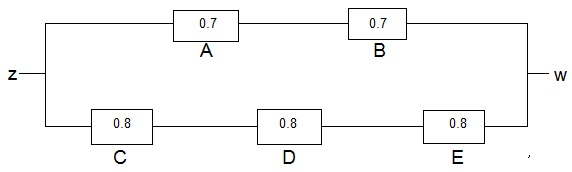
\includegraphics[width=.50\textwidth]{tab3}
% \end{figure}